\documentclass{beamer}
\usepackage{handout}
\title{PS-1006: Politics - Introduction to Politics}
\author{Tom T. Hsiao}
\date{\today}
\begin{document}
\fontspec{Times New Roman}
\begin{frame}
\begin{center}
\Large{Chapter 1 Introduction to Politics} \\
\vspace{3em}
\normalsize{Instructor: Tzu-Chi Hsiao} \\
\vspace{3em}
\small{Department of Political Science} \\
\vspace{1em}
\small{University} \\
\end{center}
\end{frame}
\begin{frame}{Content}
\begin{itemize}
\item What is Politics?
\item The Political System
\item The State
\item The Nation
\item The Government
\end{itemize}
\end{frame}
\begin{frame}{Content}
\begin{itemize}
\item What is Politics?
\item \textcolor{gray}{The Political System}
\item \textcolor{gray}{The State}
\item \textcolor{gray}{The Nation}
\item \textcolor{gray}{The Government}
\end{itemize}
\end{frame}
\begin{frame}{System of the government I}
\begin{center}
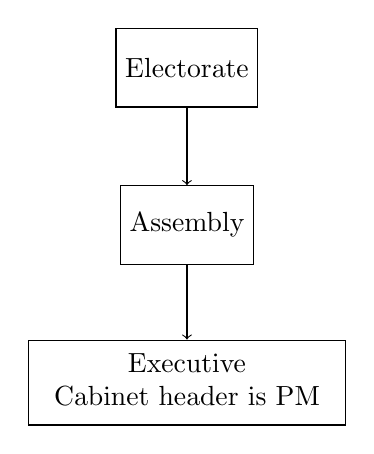
\begin{tikzpicture}
\node[draw, rectangle, minimum width=1cm, minimum height=1cm] (top) at (1, 1.5) {Electorate};
\node[draw, rectangle, minimum width=1cm, minimum height=1cm] (mid) at (1, -0.5) {Assembly};
\node[draw, rectangle, minimum width=1cm, minimum height=1cm] (bottom) at (1, -2.5) {\begin{tabular}{c} Executive \\ Cabinet header is PM \end{tabular}};
\draw[->] (top.south) -- (mid.north);
\draw[->] (mid.south) -- (bottom.north);
\end{tikzpicture}
\end{center}
\begin{center}
Parliamentary system.
\end{center}
\end{frame}
\begin{frame}{System of the government II}
\begin{center}
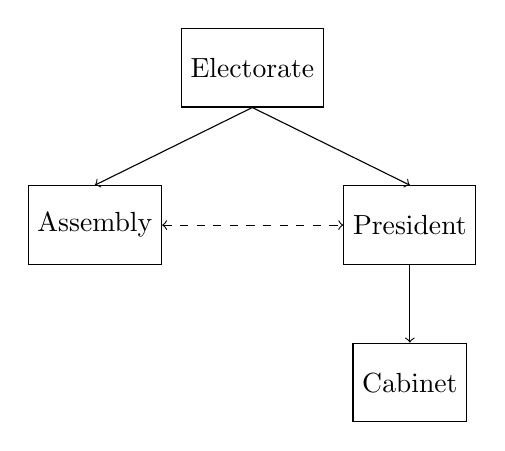
\begin{tikzpicture}
\node[draw, rectangle, minimum width=1cm, minimum height=1cm] (top) at (1, 1.5) {Electorate};
\node[draw, rectangle, minimum width=1cm, minimum height=1cm] (midL) at (-1, -0.5) {Assembly};
\node[draw, rectangle, minimum width=1cm, minimum height=1cm] (midR) at (3, -0.5) {President};
\node[draw, rectangle, minimum width=1cm, minimum height=1cm] (bottom) at (3, -2.5) {Cabinet};
\draw[->] (top.south) -- (midL.north);
\draw[->] (top.south) -- (midR.north);
\draw[->] (midR.south) -- (bottom.north) ;
\draw[<->, dashed] (midL.east) -- (midR.west);
\end{tikzpicture}
\end{center}
\begin{center}
President system.
\end{center}
\end{frame}
\begin{frame}{System of the government III}
\begin{minipage}{0.45\textwidth}
\begin{center}
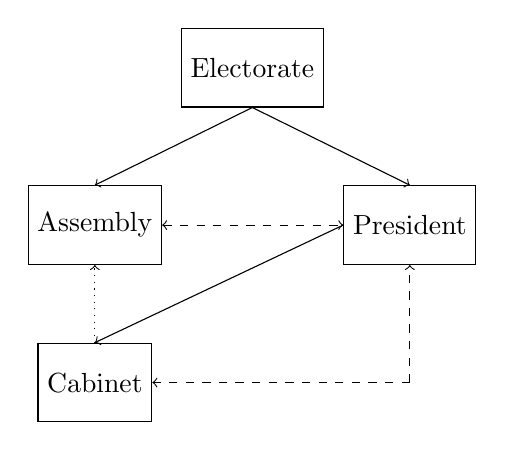
\begin{tikzpicture}
\node[draw, rectangle, minimum width=1cm, minimum height=1cm] (top) at (1, 1.5) {Electorate};
\node[draw, rectangle, minimum width=1cm, minimum height=1cm] (midL) at (-1, -0.5) {Assembly};
\node[draw, rectangle, minimum width=1cm, minimum height=1cm] (midR) at (3, -0.5) {President};
\node[draw, rectangle, minimum width=1cm, minimum height=1cm] (bottom) at (-1, -2.5) {Cabinet};
\node(1) at (3, -2.5) {};
\draw[->] (top.south) -- (midL.north);
\draw[->] (top.south) -- (midR.north);
\draw[->] (midR.west) -- (bottom.north);
\draw[->, dashed] (1.center) -- (bottom.east);
\draw[->, dashed] (1.center) -- (midR.south);
\draw[->, dotted] (bottom.north) -- (midL.south);
\draw[<->, dashed] (midL.east) -- (midR.west);
\end{tikzpicture}
\end{center}
\begin{center}
Premier-President system.
\end{center}
\end{minipage}
\hfill
\begin{minipage}{0.45\textwidth}
\begin{center}
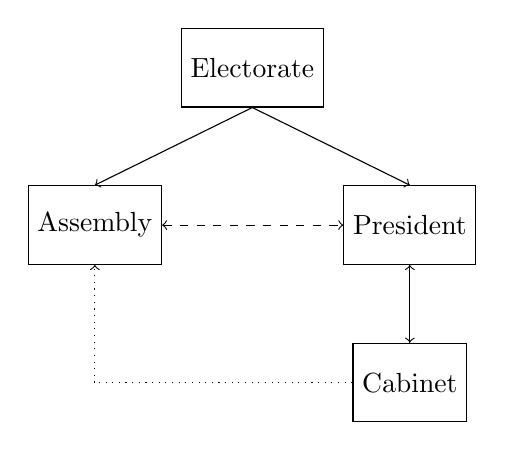
\begin{tikzpicture}
\node[draw, rectangle, minimum width=1cm, minimum height=1cm] (top) at (1, 1.5) {Electorate};
\node[draw, rectangle, minimum width=1cm, minimum height=1cm] (midL) at (-1, -0.5) {Assembly};
\node[draw, rectangle, minimum width=1cm, minimum height=1cm] (midR) at (3, -0.5) {President};
\node[draw, rectangle, minimum width=1cm, minimum height=1cm] (bottom) at (3, -2.5) {Cabinet};
\node(1) at (-1, -2.5) {};
\draw[->] (top.south) -- (midL.north);
\draw[->] (top.south) -- (midR.north);
\draw[<->, dashed] (midL.east) -- (midR.west);
\draw[->] (midR.south) -- (bottom.north);
\draw[->, dotted] (bottom.north) -- (midR.south) ;
\draw[-, dotted](bottom.west) -- (1.center);
\draw[->, dotted] (1.center) -- (midL.south);
\end{tikzpicture}
\end{center}
\begin{center}
President-parlimentary system.
\end{center}
\end{minipage}
\end{frame}
\begin{frame}{Explanation}
\begin{center}
\begin{itemize}
\item The solid line means the hierarchical relationship, with arrow indicating selection of agent by principle.
\item The dashed line with two-headed arrow indicates transactional relationship, with arrow indicating accountability of agent to principle who may terminate delegated authority.
\item The dotted line with two-headed arrow indicates transactional relationship.
\end{itemize}
\end{center}
\end{frame}
\begin{frame}{}
\begin{center}
\Large{End of Chapter 1}
\end{center}
\end{frame}
\end{document}
